\documentclass{standalone}
\usepackage{tikz}
\usetikzlibrary{patterns, positioning}
\usepackage[sfdefault]{ClearSans} %% option 'sfdefault' activates Clear Sans as the default text font
\usepackage[T1]{fontenc}

\begin{document}
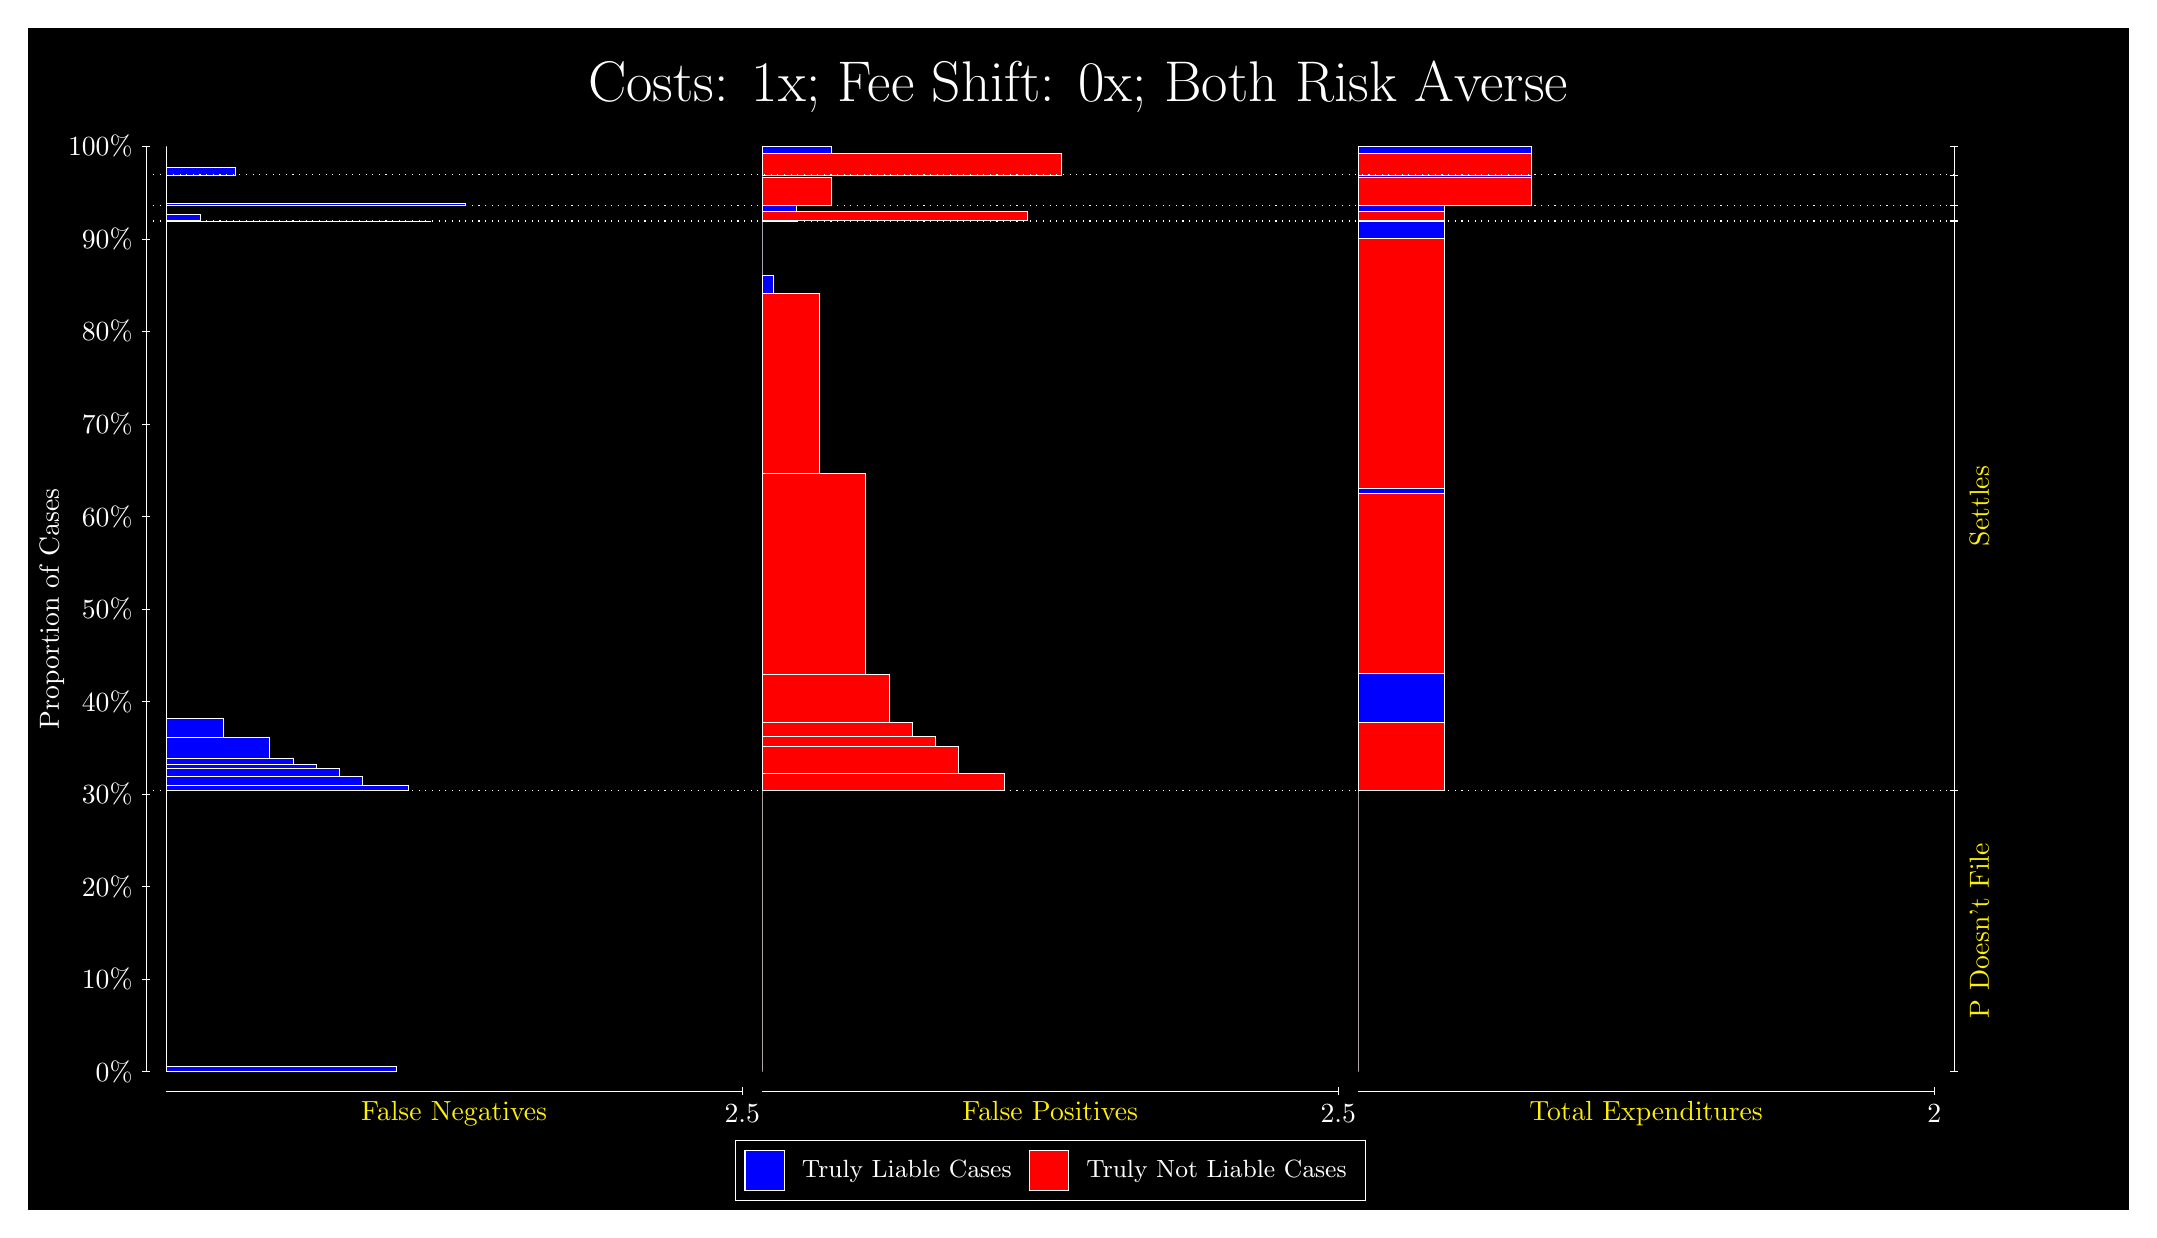
\begin{tikzpicture}
\draw[fill=black] (0,0) rectangle (26.667,15);
\draw[text=white] (0,13.5) rectangle (26.667,15) node[midway] {\huge Costs: 1x; Fee Shift: 0x; Both Risk Averse};
\draw[white, very thin] (1.5,1.75) -- (1.5,13.5);
\node[rotate=90, text=white, anchor=center] at (0.3, 7.625) {Proportion of Cases};
\draw[white, very thin] (1.45,1.75) -- (1.55,1.75);
\node[text=white, anchor=east] at (1.45, 1.75) {0\%};
\draw[white, very thin] (1.45,2.925) -- (1.55,2.925);
\node[text=white, anchor=east] at (1.45, 2.925) {10\%};
\draw[white, very thin] (1.45,4.1) -- (1.55,4.1);
\node[text=white, anchor=east] at (1.45, 4.1) {20\%};
\draw[white, very thin] (1.45,5.275) -- (1.55,5.275);
\node[text=white, anchor=east] at (1.45, 5.275) {30\%};
\draw[white, very thin] (1.45,6.45) -- (1.55,6.45);
\node[text=white, anchor=east] at (1.45, 6.45) {40\%};
\draw[white, very thin] (1.45,7.625) -- (1.55,7.625);
\node[text=white, anchor=east] at (1.45, 7.625) {50\%};
\draw[white, very thin] (1.45,8.8) -- (1.55,8.8);
\node[text=white, anchor=east] at (1.45, 8.8) {60\%};
\draw[white, very thin] (1.45,9.975) -- (1.55,9.975);
\node[text=white, anchor=east] at (1.45, 9.975) {70\%};
\draw[white, very thin] (1.45,11.15) -- (1.55,11.15);
\node[text=white, anchor=east] at (1.45, 11.15) {80\%};
\draw[white, very thin] (1.45,12.325) -- (1.55,12.325);
\node[text=white, anchor=east] at (1.45, 12.325) {90\%};
\draw[white, very thin] (1.45,13.5) -- (1.55,13.5);
\node[text=white, anchor=east] at (1.45, 13.5) {100\%};

\draw[white, very thin] (24.457,1.75) -- (24.457,13.5);
\draw[white, very thin] (24.407,1.75) -- (24.507,1.75);
\node[anchor=west] at (24.407, 1.75) {};
\draw[white, very thin] (24.407,5.3182) -- (24.507,5.3182);
\node[anchor=west] at (24.407, 5.3182) {};
\draw[white, very thin] (24.407,12.546) -- (24.507,12.546);
\node[anchor=west] at (24.407, 12.546) {};
\draw[white, very thin] (24.407,12.561) -- (24.507,12.561);
\node[anchor=west] at (24.407, 12.561) {};
\draw[white, very thin] (24.407,12.749) -- (24.507,12.749);
\node[anchor=west] at (24.407, 12.749) {};
\draw[white, very thin] (24.407,13.138) -- (24.507,13.138);
\node[anchor=west] at (24.407, 13.138) {};
\draw[white, very thin] (24.407,13.5) -- (24.507,13.5);
\node[anchor=west] at (24.407, 13.5) {};

\draw[white, very thin, fill=blue] (1.75,1.75) rectangle (4.6775,1.8133);
\draw[white, very thin, fill=red] (1.75,1.8133) rectangle (1.75,5.3182);
\draw[white, very thin, fill=blue] (1.75,5.3182) rectangle (4.8239,5.3914);
\draw[white, very thin, fill=blue] (1.75,5.3914) rectangle (4.2384,5.4988);
\draw[white, very thin, fill=blue] (1.75,5.4988) rectangle (3.9457,5.6024);
\draw[white, very thin, fill=blue] (1.75,5.6024) rectangle (3.6529,5.6514);
\draw[white, very thin, fill=blue] (1.75,5.6514) rectangle (3.3602,5.7298);
\draw[white, very thin, fill=blue] (1.75,5.7298) rectangle (3.0674,6.0013);
\draw[white, very thin, fill=blue] (1.75,6.0013) rectangle (2.4819,6.2325);
\draw[white, very thin, fill=red] (1.75,6.2325) rectangle (1.75,12.546);
\draw[white, very thin, fill=blue] (1.75,12.546) rectangle (5.1167,12.546);
\draw[white, very thin, fill=red] (1.75,12.546) rectangle (1.75,12.561);
\draw[white, very thin, fill=blue] (1.75,12.561) rectangle (2.1891,12.637);
\draw[white, very thin, fill=red] (1.75,12.637) rectangle (1.75,12.749);
\draw[white, very thin, fill=blue] (1.75,12.749) rectangle (5.5558,12.779);
\draw[white, very thin, fill=red] (1.75,12.779) rectangle (1.75,13.138);
\draw[white, very thin, fill=blue] (1.75,13.138) rectangle (2.6283,13.229);
\draw[white, very thin, fill=red] (1.75,13.229) rectangle (1.75,13.5);
\draw[white, very thin, fill=red] (9.3189,1.75) rectangle (9.3189,5.2549);
\draw[white, very thin, fill=blue] (9.3189,5.2549) rectangle (9.3189,5.3182);
\draw[white, very thin, fill=red] (9.3189,5.3182) rectangle (12.393,5.5415);
\draw[white, very thin, fill=red] (9.3189,5.5415) rectangle (11.807,5.8821);
\draw[white, very thin, fill=red] (9.3189,5.8821) rectangle (11.515,6.011);
\draw[white, very thin, fill=red] (9.3189,6.011) rectangle (11.222,6.1808);
\draw[white, very thin, fill=red] (9.3189,6.1808) rectangle (10.929,6.8003);
\draw[white, very thin, fill=red] (9.3189,6.8003) rectangle (10.636,9.3523);
\draw[white, very thin, fill=red] (9.3189,9.3523) rectangle (10.051,11.631);
\draw[white, very thin, fill=blue] (9.3189,11.631) rectangle (9.4652,11.862);
\draw[white, very thin, fill=blue] (9.3189,11.862) rectangle (9.3189,12.546);
\draw[white, very thin, fill=red] (9.3189,12.546) rectangle (9.758,12.56);
\draw[white, very thin, fill=blue] (9.3189,12.56) rectangle (9.3189,12.561);
\draw[white, very thin, fill=red] (9.3189,12.561) rectangle (12.686,12.674);
\draw[white, very thin, fill=blue] (9.3189,12.674) rectangle (9.758,12.749);
\draw[white, very thin, fill=red] (9.3189,12.749) rectangle (10.197,13.108);
\draw[white, very thin, fill=blue] (9.3189,13.108) rectangle (9.3189,13.138);
\draw[white, very thin, fill=red] (9.3189,13.138) rectangle (13.125,13.409);
\draw[white, very thin, fill=blue] (9.3189,13.409) rectangle (10.197,13.5);
\draw[white, very thin, fill=red] (16.888,1.75) rectangle (16.888,5.2549);
\draw[white, very thin, fill=blue] (16.888,5.2549) rectangle (16.888,5.3182);
\draw[white, very thin, fill=red] (16.888,5.3182) rectangle (17.986,6.1808);
\draw[white, very thin, fill=blue] (16.888,6.1808) rectangle (17.986,6.8109);
\draw[white, very thin, fill=red] (16.888,6.8109) rectangle (17.986,9.0898);
\draw[white, very thin, fill=blue] (16.888,9.0898) rectangle (17.986,9.1631);
\draw[white, very thin, fill=red] (16.888,9.1631) rectangle (17.986,12.334);
\draw[white, very thin, fill=blue] (16.888,12.334) rectangle (17.986,12.546);
\draw[white, very thin, fill=red] (16.888,12.546) rectangle (17.986,12.56);
\draw[white, very thin, fill=blue] (16.888,12.56) rectangle (17.986,12.561);
\draw[white, very thin, fill=red] (16.888,12.561) rectangle (17.986,12.674);
\draw[white, very thin, fill=blue] (16.888,12.674) rectangle (17.986,12.749);
\draw[white, very thin, fill=red] (16.888,12.749) rectangle (19.083,13.108);
\draw[white, very thin, fill=blue] (16.888,13.108) rectangle (19.083,13.138);
\draw[white, very thin, fill=red] (16.888,13.138) rectangle (19.083,13.409);
\draw[white, very thin, fill=blue] (16.888,13.409) rectangle (19.083,13.5);
\draw[white, dotted] (1.5,5.3182) -- (24.457,5.3182);
\draw[white, dotted] (1.5,12.546) -- (24.457,12.546);
\draw[white, dotted] (1.5,12.561) -- (24.457,12.561);
\draw[white, dotted] (1.5,12.749) -- (24.457,12.749);
\draw[white, dotted] (1.5,13.138) -- (24.457,13.138);
\draw[white, very thin] (1.75,1.5) -- (9.0689,1.5);
\node[text=yellow, anchor=north] at (5.4094, 1.5) {False Negatives};
\draw[white, very thin] (9.0689,1.45) -- (9.0689,1.55);
\node[text=white, anchor=north] at (9.0689, 1.45) {2.5};

\draw[white, very thin] (9.3189,1.5) -- (16.638,1.5);
\node[text=yellow, anchor=north] at (12.978, 1.5) {False Positives};
\draw[white, very thin] (16.638,1.45) -- (16.638,1.55);
\node[text=white, anchor=north] at (16.638, 1.45) {2.5};

\draw[white, very thin] (16.888,1.5) -- (24.207,1.5);
\node[text=yellow, anchor=north] at (20.547, 1.5) {Total Expenditures};
\draw[white, very thin] (24.207,1.45) -- (24.207,1.55);
\node[text=white, anchor=north] at (24.207, 1.45) {2};

\node[text=yellow, centered, rotate=90] at (24.777, 3.5341) {P Doesn't File};
\node[text=yellow, centered, rotate=90] at (24.777, 8.9318) {Settles};





\draw (12.978300999999998,1.5) node[draw=none] (baseCoordinate) {};
\begin{scope}[align=center]
        \matrix[scale=0.5, draw=white, below=0.5cm of baseCoordinate, nodes={draw}, column sep=0.1cm]{
            \node[rectangle, draw, minimum width=0.5cm, minimum height=0.5cm, fill=blue] {}; &
            \node[draw=none, font=\small, text=white] (B) {Truly Liable Cases}; &
            \node[rectangle, draw, minimum width=0.5cm, minimum height=0.5cm, fill=red] {}; &
            \node[draw=none, font=\small, text=white] (B) {Truly Not Liable Cases}; \\
            };
\end{scope}

\end{tikzpicture}
\end{document}